%=====================================================================
\section{Extended Empirical Analysis}\label{sec:empirical}
%=====================================================================

The headline results in Sections~\ref{sec:m1}--\ref{sec:results} are pooled over seasons.
Pooling is convenient but can hide regime changes, heterogeneous identification, and the fact
that judges and fans separate different couples. This section reopens the reconstructed panel
and reports six additional analyses, all computed from the materialized CSV files. The complete
season-level table is deferred to Appendix~\ref{app:seasons} so that the narrative is not
interrupted by a 34-row table.

\subsection{Season-by-Season Dynamics}\label{sec:season_dynamics}

Figure~\ref{fig:seasondyn} plots four quantities by season. Panel~(a) shows that the mean judge
share and mean reconstructed fan share track each other closely, but that the fan share is
systematically lower and more volatile --- consistent with the uniform maximum-entropy posterior
spreading mass across the feasible set. Panel~(b) shows that mean credible-interval width is
highest in the short early seasons ($0.446$ in the rank era) and declines to $0.332$ in the
percent era and $0.306$ in the bottom-two era; the early seasons have small fields, so each
couple's feasible share range is large in absolute terms.

\begin{figure}[H]
\centering
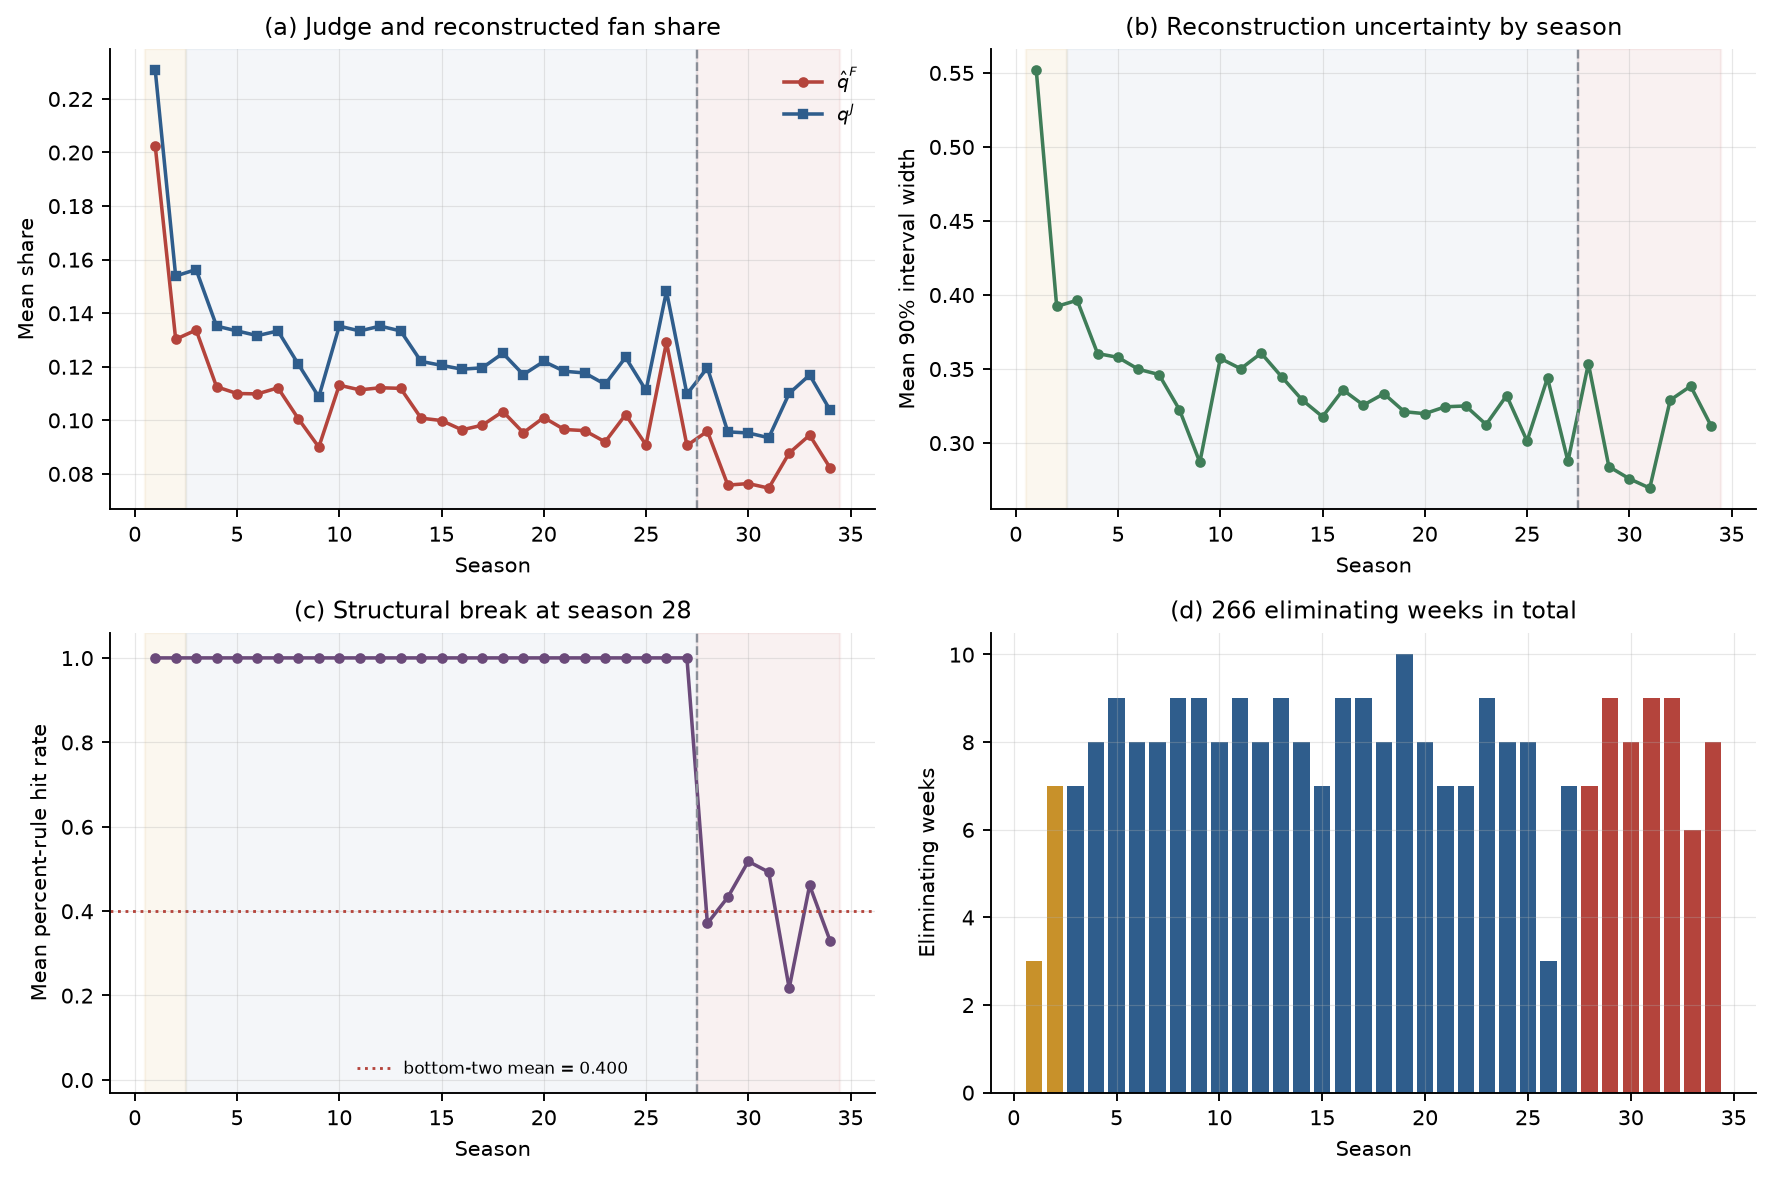
\includegraphics[width=0.94\textwidth]{figures_ext/fig03_season_dynamics.png}
\caption{Season-level dynamics. (a) Mean judge share and mean reconstructed fan share.
(b) Mean $90\%$ credible-interval width. (c) Mean percent-rule hit rate over eliminating
weeks; the dashed line marks the $0.400$ bottom-two average. (d) Number of eliminating weeks
per season ($266$ in total). Shaded bands mark the three fusion regimes.}
\label{fig:seasondyn}
\end{figure}

Panel~(c) is the sharpest descriptive result: the hit rate is exactly $1.000$ in every season
from $1$ through $27$ and drops abruptly to between $0.37$ and $0.43$ from season $28$ onward.
There is no gradual drift. Panel~(d) confirms that this is not a sample-size artefact --- the
late seasons actually contribute \emph{more} eliminating weeks than the early ones. A complete
season-by-season breakdown including couple--weeks, mean shares, mean interval width and worst
split-$\hat R$ is given in Table~\ref{tab:seasonstats}.

\subsection{The Structure of Uncertainty}\label{sec:uncertainty}

The problem asks explicitly whether the certainty of the estimated fan vote is always the
same. It is not, but the \emph{direction} of the heterogeneity is subtler than a first reading
suggests, and it depends on whether width is measured in absolute or field-size-normalised
terms.

Across all $2{,}777$ couple--weeks the $90\%$ interval width $\Delta$ has mean $0.328$,
median $0.313$, $5$th percentile $0.065$ and $95$th percentile $0.607$, with a full range of
$0.022$ to $0.898$. The posterior standard deviation has mean $0.088$. Regressing (in the
sense of raw correlation) $\Delta$ on the weekly design variables gives
$r=-0.649$ against the number of surviving couples, $r=+0.563$ against competition week,
$r=-0.427$ against the number of active constraints, and $r=+0.143$ against the within-week
standard deviation of judge shares. In \emph{absolute} terms, therefore, the widest intervals
occur late in the season in small fields, where each surviving couple commands a large share
and the simplex face is wide. This is the opposite of the naive expectation that large fields
are harder to identify.

That apparent paradox is a scale effect. Rescaling by field size,
$\Delta^{\rm rel}=n_{sw}\Delta$ (mean $2.833$), reverses two of the signs:
$r=+0.261$ against field size and $r=-0.241$ against week. On a comparable scale, large
early-season fields \emph{are} the least identified, exactly as the intuition predicts.
Figure~\ref{fig:uncstruct} shows both measures side by side, and
Tables~\ref{tab:uncertaintyweeks} and~\ref{tab:judgebaseline} give the week-by-week and
field-size breakdowns. We therefore recommend that any operational use of these estimates
report $\Delta^{\rm rel}$ alongside $\Delta$; the absolute width alone can be misleading.

\begin{figure}[H]
\centering
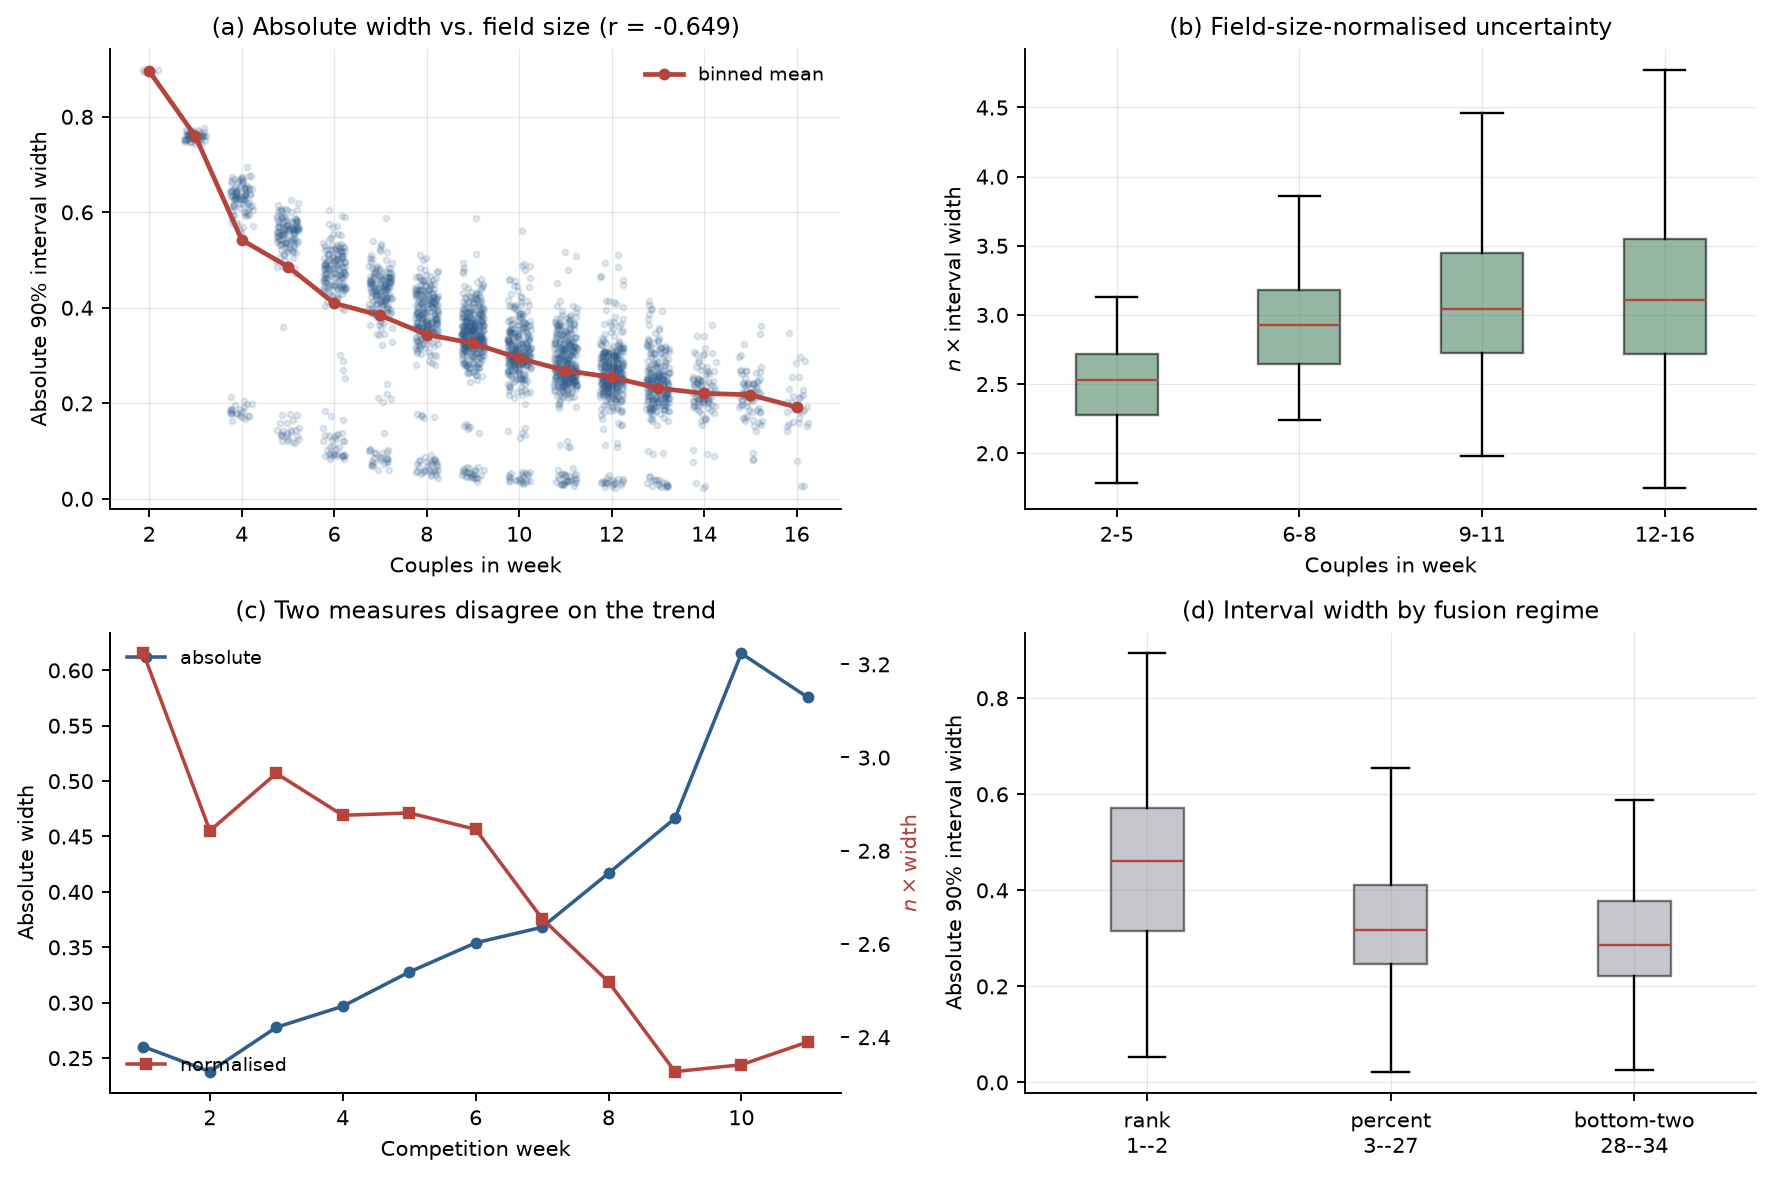
\includegraphics[width=0.94\textwidth]{figures_ext/fig04_uncertainty_structure.png}
\caption{What drives reconstruction uncertainty. (a) Absolute interval width against field
size with binned means. (b) Field-size-normalised width by field-size stratum. (c) Absolute
(left axis) and normalised (right axis) width by competition week --- the two trend in opposite
directions. (d) Absolute width by fusion regime.}
\label{fig:uncstruct}
\end{figure}

% AUTO-GENERATED table — values computed by analyze_extended.py
\begin{table}[H]
\centering
\caption{Uncertainty by competition week. $\overline{\Delta}$ is the mean absolute $90\%$ credible-interval width; $\overline{\Delta}_{\rm rel}=n\,\overline{\Delta}$ rescales it by the field size so that intervals are comparable across weeks with different numbers of surviving couples. Absolute width grows late in a season because shares themselves grow; the rescaled width is the comparable measure.}
\label{tab:uncertaintyweeks}
\begin{tabular}{lrrrrr}
\toprule
Week & $n$ & Couples & $\overline{q^F}$ & $\overline{\Delta}$ & $\overline{\Delta}_{\rm rel}$ \\ 
\midrule
1 & 421 & 12.6 & 0.061 & 0.260 & 3.22 \\ 
2 & 404 & 12.2 & 0.067 & 0.238 & 2.84 \\ 
3 & 360 & 10.9 & 0.075 & 0.278 & 2.97 \\ 
4 & 326 & 10.0 & 0.084 & 0.297 & 2.88 \\ 
5 & 288 & 9.0 & 0.092 & 0.328 & 2.88 \\ 
6 & 261 & 8.3 & 0.103 & 0.354 & 2.85 \\ 
7 & 228 & 7.3 & 0.117 & 0.368 & 2.65 \\ 
8 & 191 & 6.2 & 0.143 & 0.417 & 2.52 \\ 
9 & 152 & 5.1 & 0.179 & 0.466 & 2.33 \\ 
10 & 109 & 4.0 & 0.238 & 0.615 & 2.34 \\ 
11 & 37 & 4.2 & 0.214 & 0.576 & 2.39 \\ 
\bottomrule
\end{tabular}
\end{table}


\subsection{Judge--Fan Disagreement in the Fine Ordering}

Figure~\ref{fig:channels} decomposes the $0.832$ level correlation and $0.153$ rank-vector
correlation into interpretable quantities. Panel~(a) plots $q^J$ against $\tilde q^F$; the
cloud follows the diagonal but with substantial scatter. Panel~(b) plots the within-week
reallocation $\tilde q^F-q^J$, which has mean zero \emph{by construction} (both vectors sum to
one within a week) but standard deviation $0.040$, with $5$th and $95$th percentiles of
$-0.080$ and $+0.057$. The dispersion is largest in the rank era ($0.060$), intermediate in
the percent era ($0.044$) and smallest in the bottom-two era ($0.024$) --- evidence that the
later rules compress the scope for fan-driven reallocation.

Panel~(c) is the more telling diagnostic: the absolute difference $|r^F-r^J|$ has mean
$3.27$ rank positions, median $2.5$, $90$th percentile $7$, and exceeds one position in
$65.8\%$ of all couple--weeks. In other words, for roughly two thirds of couple--weeks the
audience and the panel place the couple at least two ordinal positions apart. This is the
mechanical source of rule sensitivity: rank fusion is a function of these disagreeing ordinal
vectors, while percent fusion is a function of the largely agreeing share levels.

\begin{figure}[H]
\centering
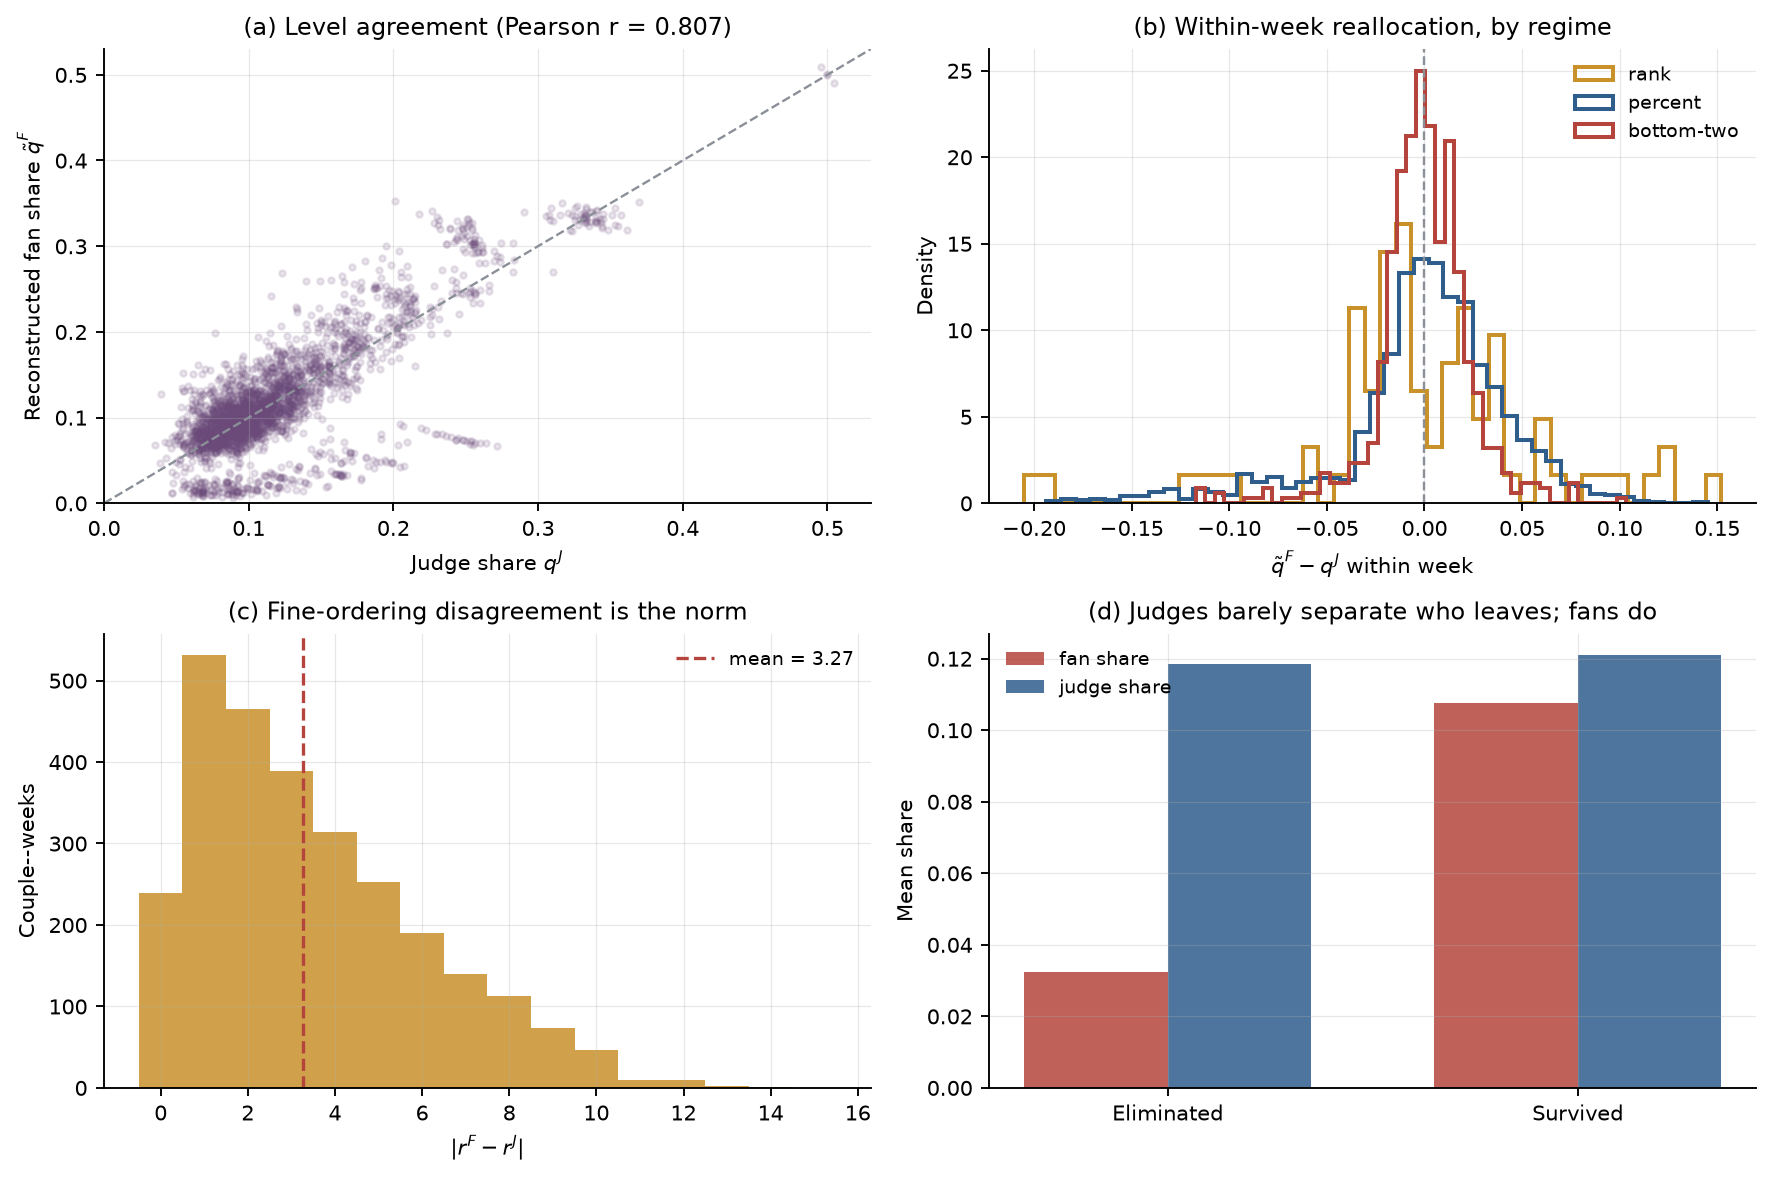
\includegraphics[width=0.94\textwidth]{figures_ext/fig05_judge_fan_channels.png}
\caption{Judge and fan channels. (a) Judge share versus renormalised fan share, with the
identity line. (b) Within-week reallocation $\tilde q^F-q^J$ by fusion regime. (c) Absolute
rank displacement $|r^F-r^J|$. (d) Mean share levels for eliminated versus surviving couples.}
\label{fig:channels}
\end{figure}

Panel~(d) contains a result that is easy to overlook. Eliminated couples have mean fan share
$0.032$ against $0.108$ for survivors --- a $3.3$-fold separation --- but mean judge shares of
$0.118$ and $0.121$, essentially \emph{identical}. Their mean interval width is also far
narrower ($0.091$ versus $0.358$) because the elimination constraint pins the eliminated
couple near the bottom of the polytope. Thus the judge channel alone barely distinguishes who
goes home, while the reconstructed fan channel does. We stress that the latter separation is
partly structural (the polytope enforces it); the next subsection therefore isolates a
\emph{non-circular} benchmark.

\subsection{A Non-Circular Benchmark: the Judge-Only Baseline}\label{sec:judgebaseline}

Because Model~1's feasible polytope is constructed to contain the observed elimination, its
near-perfect hit rate in seasons 1--27 cannot be read as predictive accuracy. A clean,
non-circular benchmark is available without any reconstructed quantity at all: in each
eliminating week, ask whether the couple with the \emph{lowest judge share} is the one actually
eliminated. This uses only the official scores.

The answer is $\mathbf{0.444}$ pooled over all $266$ eliminating weeks. Stratifying by regime
gives $0.400$ in the rank era ($10$ weeks), $0.460$ in the percent era ($200$ weeks) and
$0.393$ in the bottom-two era ($56$ weeks). Equivalently, the eliminated couple holds the
worst judge rank in only $42.2\%$ of eliminations and sits at mean normalised judge rank
$0.781$ (where $1$ denotes the worst). Judge scores alone therefore fail to identify the
elimination in a clear majority of weeks, in \emph{every} regime. This is the cleanest
model-free evidence that a second channel --- the audience vote, and in later seasons the
judge save --- is necessary to explain outcomes.

\begin{figure}[H]
\centering
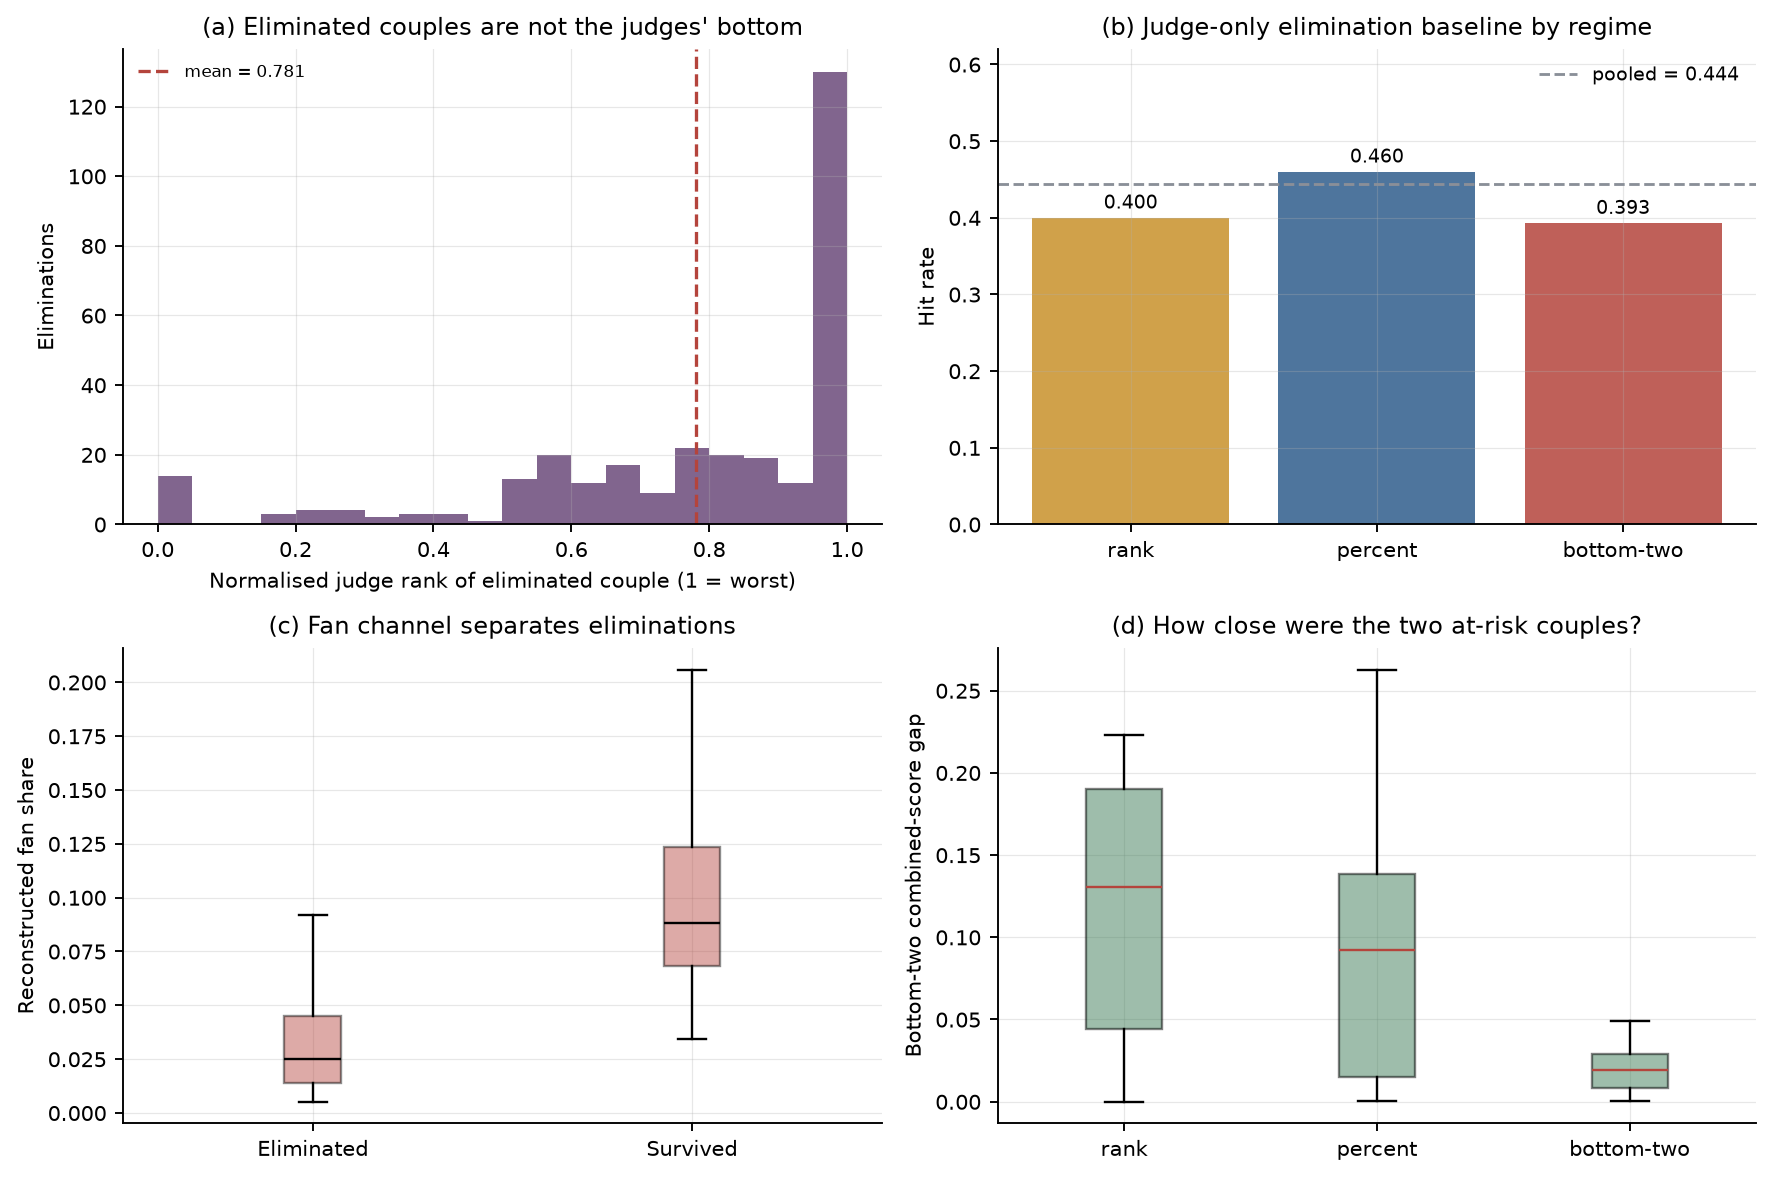
\includegraphics[width=0.94\textwidth]{figures_ext/fig06_elimination_evidence.png}
\caption{Non-circular elimination evidence. (a) Normalised judge rank of eliminated couples.
(b) Judge-only hit rate by regime, with the pooled $0.444$ line. (c) Reconstructed fan share
for eliminated versus surviving couples. (d) Gap between the two lowest combined scores by
regime (bottom-two margin distribution).}
\label{fig:elimevidence}
\end{figure}

% AUTO-GENERATED table — values computed by analyze_extended.py
\begin{table}[H]
\centering
\caption{Uncertainty by field size, and the judge-only elimination baseline. ``Judge-only hit'' is the fraction of eliminating weeks in which the couple with the lowest judge share is the one actually eliminated --- a non-circular benchmark because it uses no reconstructed fan share.}
\label{tab:judgebaseline}
\begin{tabular}{lrrrr}
\toprule
Stratum & $n$ & $\overline{\Delta}$ & $\overline{\Delta}_{\rm rel}$ & Judge-only hit \\ 
\midrule
\multicolumn{5}{l}{\emph{Field size}} \\ 
2-5 couples & 322 & 0.559 & 2.30 & -- \\ 
6-8 couples & 654 & 0.374 & 2.65 & -- \\ 
9-11 couples & 1001 & 0.297 & 2.94 & -- \\ 
12-16 couples & 800 & 0.237 & 3.06 & -- \\ 
\midrule
\multicolumn{5}{l}{\emph{Fusion regime}} \\ 
rank & 10 & -- & -- & 0.400 \\ 
percent & 200 & -- & -- & 0.460 \\ 
bottom-two & 56 & -- & -- & 0.393 \\ 
\bottomrule
\end{tabular}
\end{table}


Figure~\ref{fig:elimevidence}(d) adds a useful qualification: the gap between the two lowest
percent-combined scores is small in the bottom-two regime, so the judge save typically decides
between genuinely close couples. This is consistent with interpreting the save as a
\emph{bounded} merit safeguard rather than an arbitrary override, and it qualifies the
stronger claim one might otherwise draw from the $0.400$ hit rate.

\subsection{Trajectories of the Four Named Controversies}\label{sec:trajectories}

Table~\ref{tab:controversy} reports final-week quantities for the four contestants named in the
problem. Figure~\ref{fig:trajectories} shows their full week-by-week paths, which reveal how
those final values arose. All four carry a persistent fan premium: $\tilde q^F$ exceeds $q^J$
in $6$ of $8$ weeks for Jerry Rice, $7$ of $8$ for Billy Ray Cyrus, $9$ of $10$ for Bristol
Palin and $8$ of $9$ for Bobby Bones. Their mean judge ranks over those runs are $4.69$,
$6.88$, $6.00$ and $7.22$ respectively --- Palin and Bones spent most of their seasons in the
bottom half of the judges' ordering while retaining above-average audience support.

\begin{figure}[H]
\centering
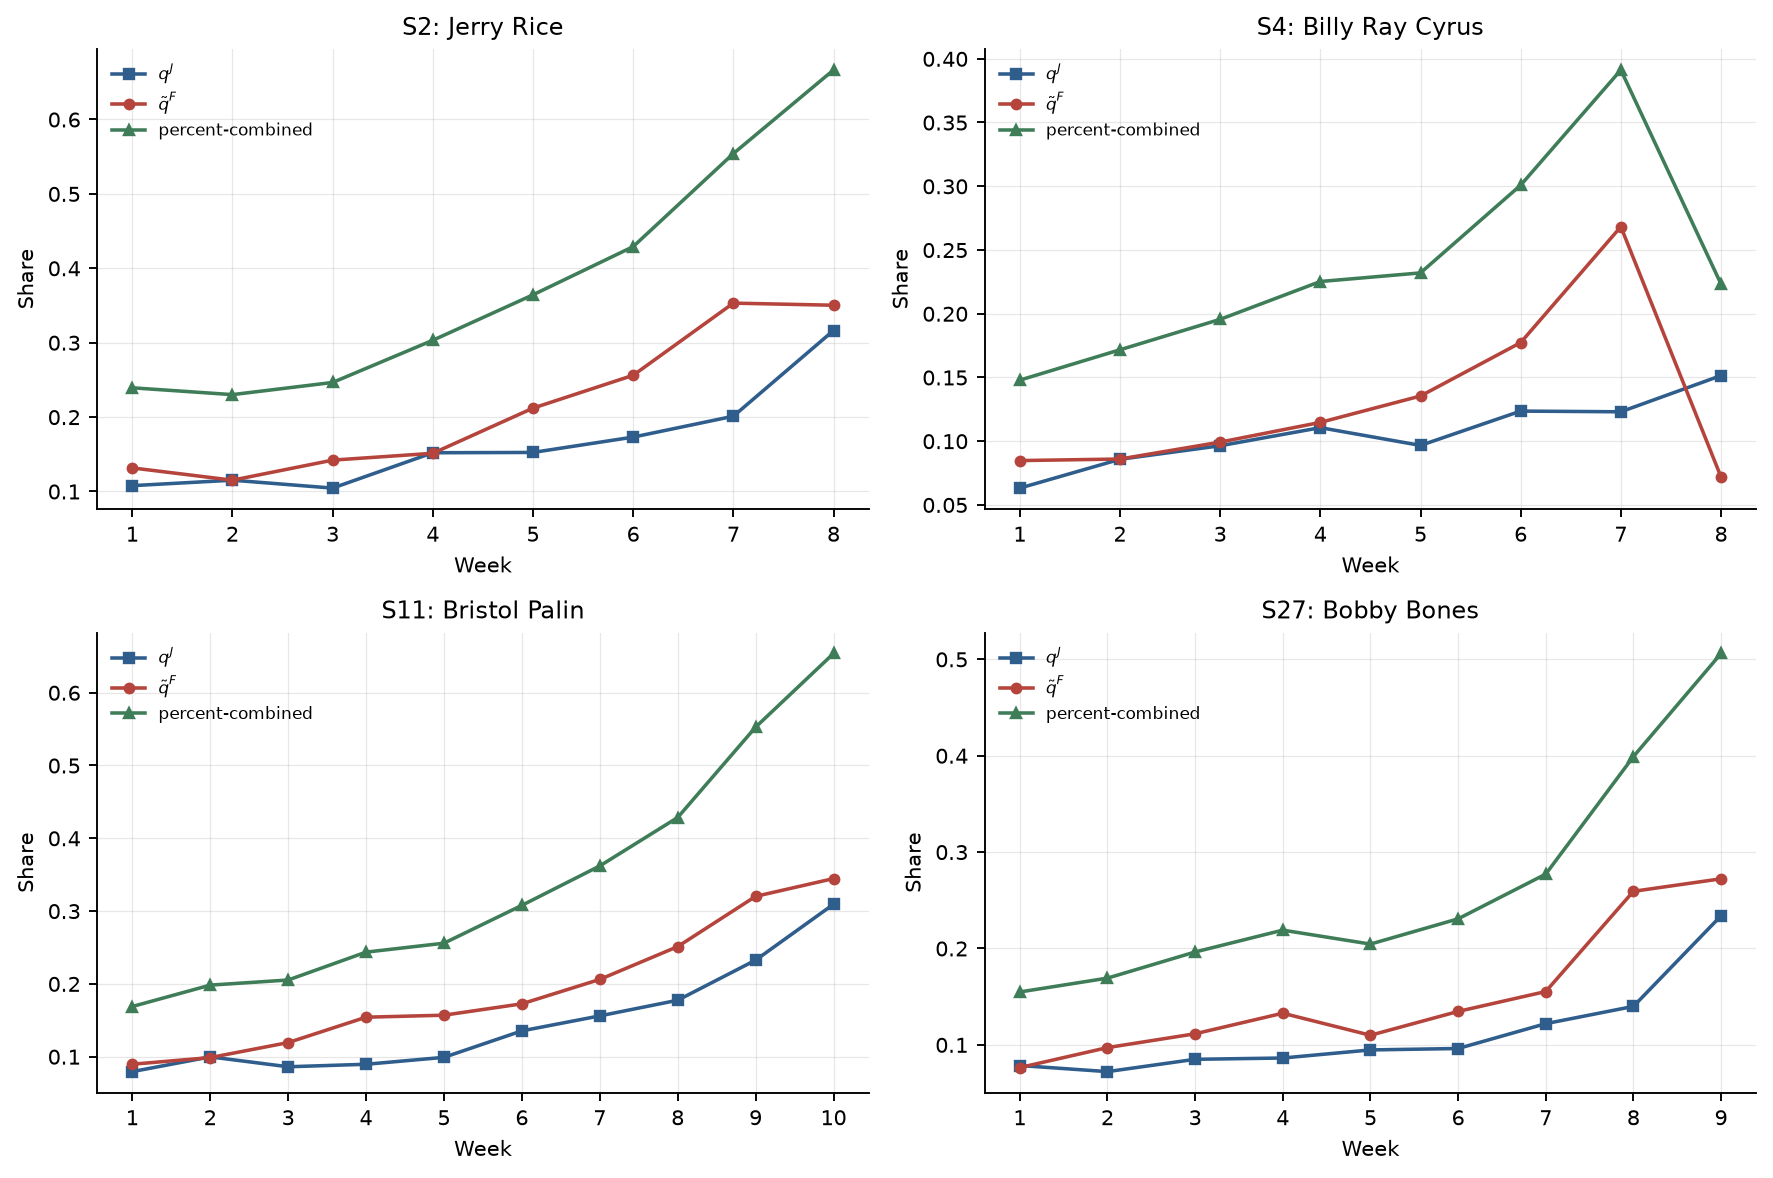
\includegraphics[width=0.94\textwidth]{figures_ext/fig11_controversy_trajectories.png}
\caption{Weekly trajectories of the four named controversy contestants. Blue squares: judge
share $q^J$; red circles: renormalised reconstructed fan share $\tilde q^F$; green triangles:
percent-combined score. The persistent red-above-blue gap is the signature of a fan-driven
survival, not a single-week anomaly.}
\label{fig:trajectories}
\end{figure}

Mean renormalised fan shares are $0.214$ (Rice), $0.130$ (Cyrus), $0.191$ (Palin) and $0.150$
(Bones), against mean judge shares of $0.165$, $0.106$, $0.146$ and $0.112$. Cyrus is the
outlier: his fan premium is positive but small, which is why rank fusion does not rescue him
whereas it does rescue the other three. The trajectories therefore corroborate, with
season-long rather than final-week evidence, the conclusion of Section~\ref{sec:results}.

\subsection{Covariate Channels and Casting Effects}\label{sec:covariates}

Model~3 decomposes the two channels by celebrity covariates. Figure~\ref{fig:covariates} and
Table~\ref{tab:covariates} extend that analysis with age bands, industry groups and
professional-partner effects. Age is negatively associated with \emph{both} channels
(Pearson $r=-0.166$ for fan share, $-0.244$ for judge share), so the fan-specific age penalty
is smaller than the raw fan--age correlation suggests: the judge channel declines at least as
steeply. The binned mean fan share is $0.108$ for ages $\le 26$, $0.109$ for $27$--$34$,
$0.097$ for $35$--$43$ and $0.082$ above $43$ --- a $24\%$ decline from the youngest to the
oldest quartile, with a mild non-monotone peak in the $27$--$34$ band.

Industry gaps are modest: athletes lead at $0.106$, actors and singers are near $0.100$,
television/media at $0.094$, and models trail at $0.076$. The fan--judge gap $\Delta$ is
negative for every industry group because judge shares are uniformly higher in this panel,
but its \emph{variation} across groups is small. The largest covariate effect we observe is
the professional partner: $0.120$ for Julianne Hough and $0.117$ for Derek Hough at the top
against $0.066$ for Brandon Armstrong and $0.064$ for Britt Stewart at the bottom, a ratio
close to $1.9$. Home-country status is essentially uninformative ($0.0994$ for US-based versus
$0.0986$ for non-US contestants). These magnitudes justify the paper's conclusion that
demographics are secondary to dance quality and partner effects.

\begin{figure}[H]
\centering
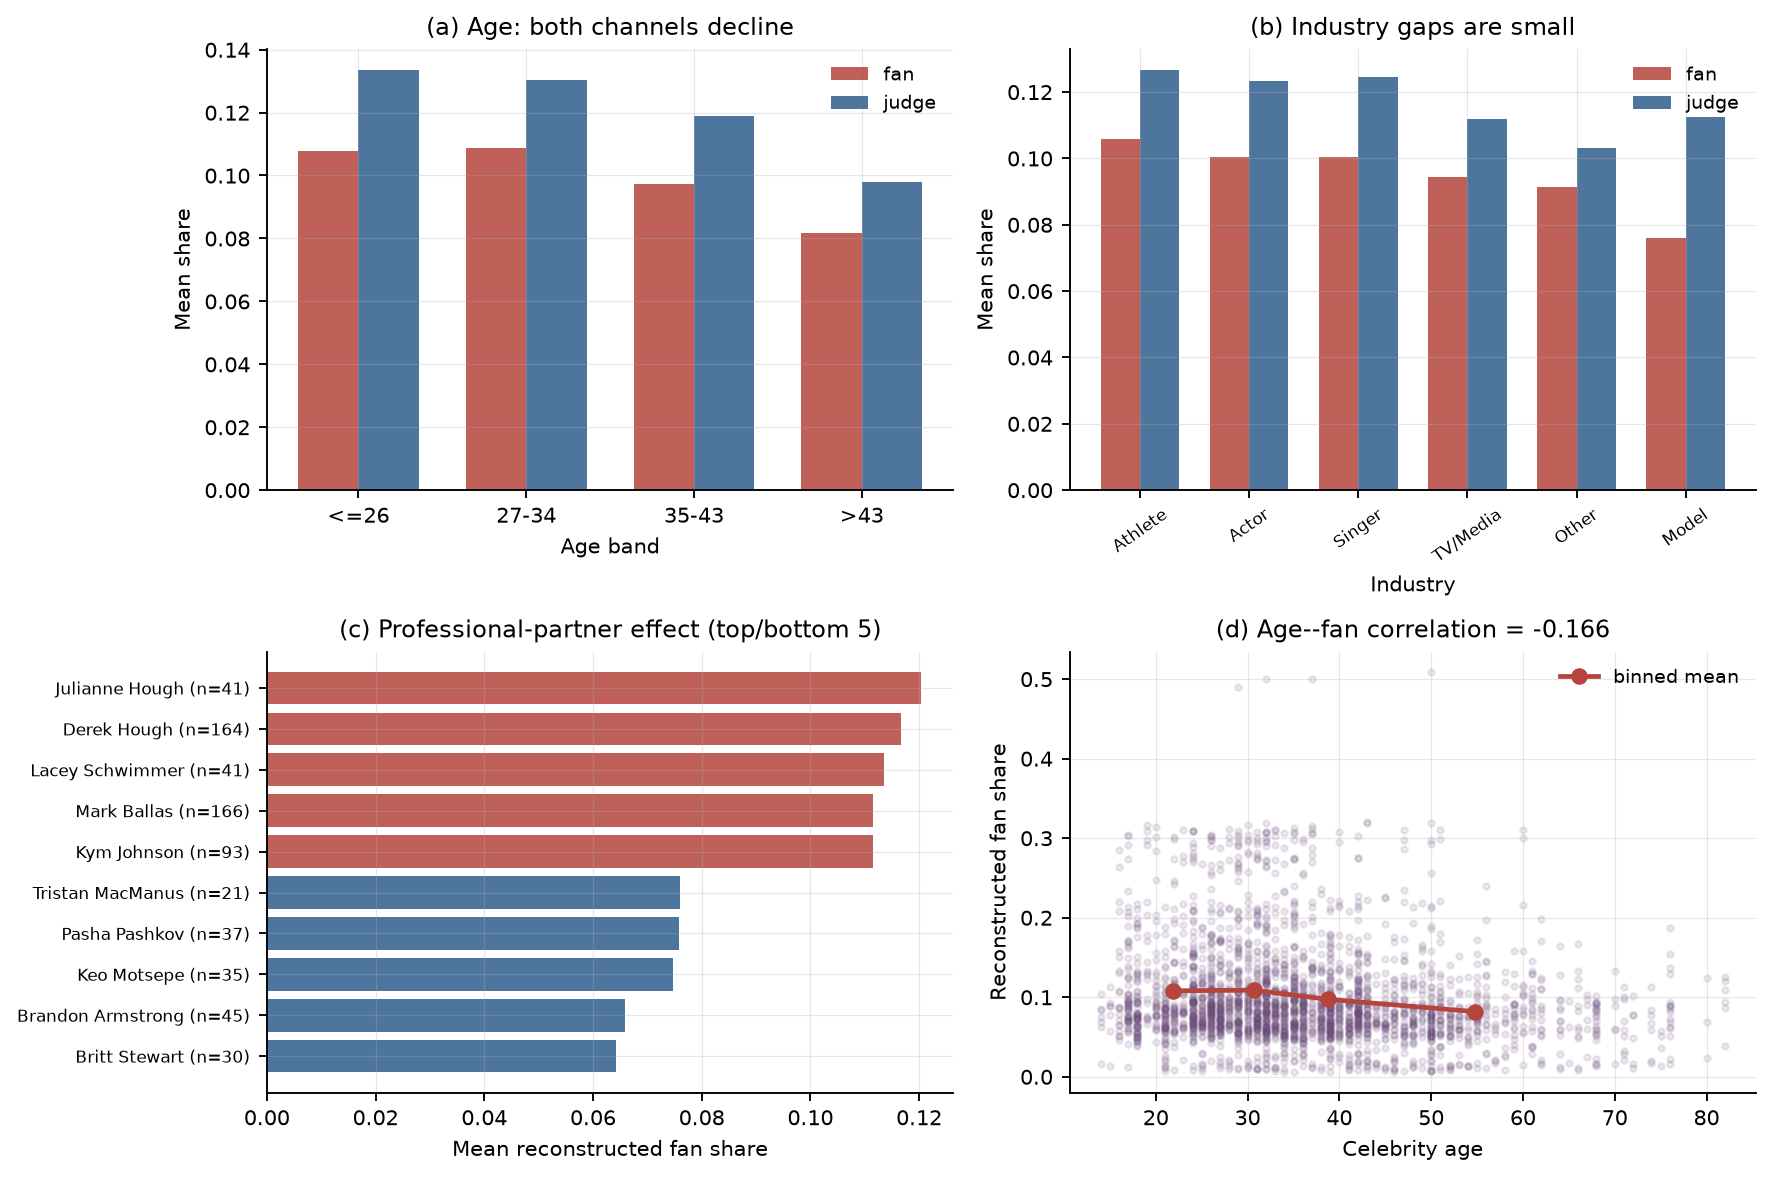
\includegraphics[width=0.94\textwidth]{figures_ext/fig12_covariate_channels.png}
\caption{Covariate channel comparison. (a) Fan and judge mean shares by age band.
(b) By industry group (groups with at least 25 couple--weeks). (c) Mean reconstructed fan
share for the five highest and five lowest professional partners with at least 20 couple--weeks.
(d) Age versus fan share with binned means.}
\label{fig:covariates}
\end{figure}

% AUTO-GENERATED table — values computed by analyze_extended.py
\begin{table}[H]
\centering
\caption{Covariate channel comparison (Model 3 panel). Mean reconstructed fan share and judge share by celebrity age band and by industry group (groups with at least 25 couple--weeks). $\Delta=\overline{q^F}-\overline{q^J}$ isolates the fan-specific premium.}
\label{tab:covariates}
\begin{tabular}{lrrrr}
\toprule
Group & $n$ & $\overline{q^F}$ & $\overline{q^J}$ & $\Delta$ \\ 
\midrule
\multicolumn{5}{l}{\emph{Age band}} \\ 
<=26 & 670 & 0.108 & 0.134 & -0.026 \\ 
27-34 & 755 & 0.109 & 0.130 & -0.022 \\ 
35-43 & 697 & 0.097 & 0.119 & -0.022 \\ 
>43 & 655 & 0.082 & 0.098 & -0.016 \\ 
\midrule
\multicolumn{5}{l}{\emph{Industry}} \\ 
Athlete & 658 & 0.106 & 0.127 & -0.021 \\ 
Actor & 882 & 0.100 & 0.123 & -0.023 \\ 
Singer & 414 & 0.100 & 0.125 & -0.024 \\ 
TV/Media & 660 & 0.094 & 0.112 & -0.017 \\ 
Other & 87 & 0.091 & 0.103 & -0.012 \\ 
Model & 76 & 0.076 & 0.112 & -0.036 \\ 
\bottomrule
\end{tabular}
\end{table}


\subsection{Regime-Level Summary}\label{sec:regimesummary}

Table~\ref{tab:erastats} consolidates the three regimes. The transition from $210$
non-bottom-two eliminating weeks (mean hit rate $1.000$, mean Brier $0.007$) to $56$
bottom-two weeks (mean hit rate $0.400$, mean Brier $0.547$) is a $0.593$ absolute drop in
hit rate and an almost eighty-fold increase in Brier score, while mean credible-interval width
barely moves ($0.332$ to $0.306$). The failure is therefore attributable to the \emph{rule},
not to a deterioration in the quality of the reconstruction. This distinction is essential to
the interpretation offered in Section~\ref{sec:discussion}.

% AUTO-GENERATED table — values computed by analyze_extended.py
\begin{table}[H]
\centering
\caption{Regime comparison. Hit rate and $\kappa$ are averaged over eliminating weeks; credible-interval width is averaged over all couple--weeks in the regime.}
\label{tab:erastats}
\begin{tabular}{lrrrrrr}
\toprule
Regime & C--W & Weeks & Elim. & Hit rate & $\overline{\Delta}$ & Brier \\ 
\midrule
rank & 78 & 14 & 10 & 1.000 & 0.446 & 0.000 \\ 
percent & 1997 & 248 & 200 & 1.000 & 0.332 & 0.007 \\ 
bottom-two & 702 & 73 & 56 & 0.400 & 0.306 & 0.547 \\ 
\bottomrule
\end{tabular}
\end{table}


%=====================================================================
